% Corrigé de l'exercice 12_BielleManivelle.
% La correction est autonome : elle ne dépend d'aucune image extérieure.
\begin{corrigebox}[Corrigé complété]

\CorrigeQuestion{1}
Le graphe des liaisons est une chaîne fermée constituée des quatre solides
$0$, $1$, $2$ et $3$ :
\begin{center}
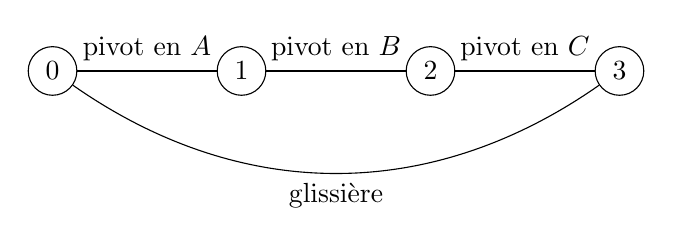
\begin{tikzpicture}[>=latex,node distance=2.4cm]
  \node[draw,circle] (S0) {$0$};
  \node[draw,circle,right of=S0] (S1) {$1$};
  \node[draw,circle,right of=S1] (S2) {$2$};
  \node[draw,circle,right of=S2] (S3) {$3$};
  \draw[-] (S0) -- node[above]{pivot en $A$} (S1);
  \draw[-] (S1) -- node[above]{pivot en $B$} (S2);
  \draw[-] (S2) -- node[above]{pivot en $C$} (S3);
  \draw[-] (S3) to[bend left=35] node[below]{glissière} (S0);
\end{tikzpicture}
\end{center}

\CorrigeQuestion{2}
On choisit $A$ comme origine et l'axe de translation de la pièce $3$ comme
axe horizontal. Pour $\theta=\dfrac{\pi}{2}$, on a
\[
B=(0,R),\qquad C=(x_C,0).
\]
La longueur $BC=L$ impose
\[
x_C^2+R^2=L^2,
\qquad
x_C=\sqrt{L^2-R^2}.
\]
Avec $R=10\,\mathrm{mm}$ et $L=20\,\mathrm{mm}$ :
\[
x_C=10\sqrt{3}\,\mathrm{mm}\simeq17{,}3\,\mathrm{mm}.
\]

\CorrigeQuestion{3}
Pour $\theta=-\dfrac{\pi}{2}$, le point $B$ est situé en $(0,-R)$.
La configuration est symétrique de la précédente par rapport à l'axe de
translation et l'on obtient encore
\[
x_C=\sqrt{L^2-R^2}=10\sqrt{3}\,\mathrm{mm}.
\]

\CorrigeQuestion{4}
Pour une position quelconque de la manivelle, la position du coulisseau est
\[
x_C(\theta)=R\cos\theta+
\sqrt{L^2-R^2\sin^2\theta}.
\]
Les positions extrêmes sont obtenues lorsque la manivelle est alignée avec
l'axe de translation :
\[
x_{\max}=L+R,
\qquad
x_{\min}=L-R.
\]
La course de la pièce $3$ vaut donc
\[
\mathcal{C}=x_{\max}-x_{\min}=2R=20\,\mathrm{mm}.
\]

\end{corrigebox}
